\section{Implementierung des Signalflusses}
Im nächsten Schritt muss der Signalfluss implementiert werden. Hierfür wird ein Ansatz der Template-Metaprogrammierung verwendet, um ein einheitliches Konzept für die Umsetzung von Signalverarbeitungsalgorithmen zu schaffen. Ebenso soll das Konzept Änderung im Singalfluss ermöglichen ohne dabei größere Eingriffe im Quellcode vornehmen zu müssen. Als Beispiel wird das folgende Blockschaltbild verwendet.
Zunächst wird eine, auf den Sensorwerten basierende, Zustandsschätzung durchgeführt. Dieser Vektor wird anschließend gefiltert und zur Berechnung des Reglers genutzt.
\begin{figure}[!h]
\centering
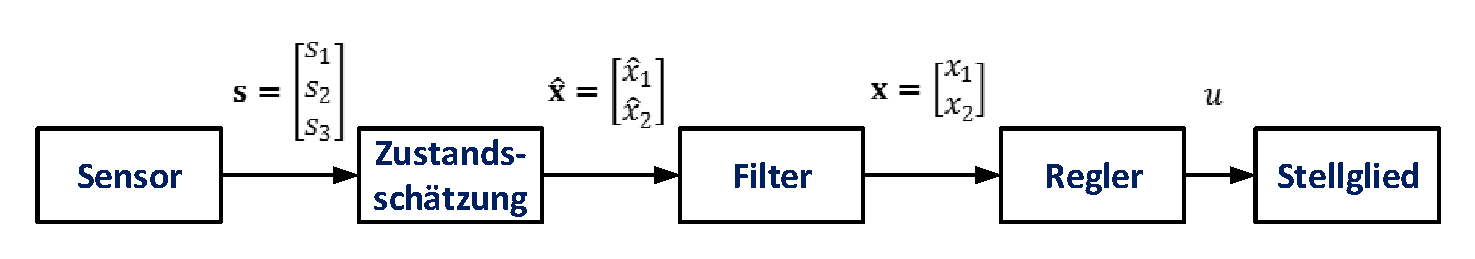
\includegraphics[width=0.9\linewidth, trim={0cm 0cm 0cm 14cm}, clip]{img/SW_1_Signalfluss_BSB.pdf}
\caption{Blockschaltbild des Signalflusses}
\end{figure}

Für die Implementierung werden die Signale als Datenobjekte implementiert. Das heißt es werden Strukturen oder Klassen entworfen, welche die Daten enthalten und ggf. Methoden für den Zugriff oder die Bearbeitung bieten. Für dieses Beispiel repräsentieren die Strukturen \textit{SSensorData} und \textit{SStateVector} den Sensor- bzw. Zustandsvektor. Für die Modellierung der Stellgröße genügt eine \textit{float}-Variable.
\begin{lstlisting}[caption={Beispielhafte Implementierung eines Datenobjektes},captionpos=b]
struct SSensorData
{
	Float32 mS1;
	Float32 mS2;
	Float32 mS3;
};
struct SStateVector
{
	Float32 mX1;
	Float32 mX2;
};
using UType = Float32;
\end{lstlisting}
Die Systeme im Signalfluss werden als Klassen implementiert, die als Aktionsobjekte bezeichnet werden. Die Klassen werden nach dem folgenden Schema entworfen, wobei als Beispiel ein Objekt zur Zustandsschätzung aufgezeigt wird.
\begin{lstlisting}[caption={Beispielhafte Implementierung eines Aktionsobjektes},captionpos=b]
class CStateEstimate
{
public:
	using InputType	 = SSensorData;
	using OutputType = SStateVector;
public:
	const OutputType& calcOutput(const InputType& input);
	const OutputType& getValue() const;
	...
private:	 
	OutputType mOutput;
};
\end{lstlisting}
Die Aktionsobjekte definieren zunächst ihren Ein- und Ausgangstyp. Die Berechnung des Systems erfolgt über die Methode \textit{calcOutput()}.
Nun müssen die Aktionsobjekte zu dem vorgegebenen Signalfluss zusammengefasst werden. Um diesen Schritt im Entwicklungsprozess zu erleichtern, soll ein Konzept implementiert werden, dem eine Typenliste der Aktionsobjekte übergeben wird und daraus das Blockschaltbild erzeugt.
Für die Implementierung der Typenliste wird der Ansatz nach \cite[S. 40 ff.]{ModernCpp} verwendet. Zunächst wird die leere Struktur \textit{CNullType} definiert, welche als Terminierungssymbol in der Typenliste fungiert. Die Liste wird mit Hilfe der Templatestruktur \textit{TTypeList} implementiert, welche als Parameter einen Anfangs- und Endtypen entgegennimmt.
\begin{lstlisting}[caption={Implementierung der Typenliste},captionpos=b]
struct CNullType{};

template<class HeadType, class TailType>
struct TTypeList
{
	using Head = HeadType;
	using Tail = TailType;
};
\end{lstlisting}
Die obige Implementierung unterstützt lediglich Listen der Länge zwei. Deshalb werden Makros verwendet \cite[S. 45]{ModernCpp}, die rekursive Intanszierungen des Templates nutzen um die Listen beliebiger Länge zu erhalten. Mittels dieser Makros kann auch die Typenliste der Aktionsobjekte erzeugt werden.
\begin{lstlisting}[caption={Definition und Aufruf der Makors für verlängerte Typenlisten},captionpos=b]
#define TYPELIST_1(T1)         TTypeList<T1, CNullType>
#define TYPELIST_2(T1, T2) 	   TTypeList<T1, TYPELIST_1(T2)>
#define TYPELIST_3(T1, T2, T3) TTypeList<T1, TYPELIST_2(T2, T3)>
...
using ActionObjList = TYPELIST_3(CStateEstimate, CFilter, CController);
\end{lstlisting}
Um nun die Aktionstypen zu einem Signalfluss-Objekt zusammenzufügen, wird das Muster der linearen Typenhierachie nach \cite[S. 62 ff.]{ModernCpp} angewandt. Dessen Aufbau erinnert an eine verkettete Liste, wobei die Typen durch Vererbung verknüpft werden. Die Templateklasse \textit{TActionHolder} wird als Träger für die Aktionsobjekte entworfen.
Im allgemeinen Fall wird dem Template der Typ eines Aktionobjektes \textit{ActionObj} und eine beliebige Elternklasse \textit{Base} übergeben, die beide an \textit{TActionHolder} vererben. In der \textit{calcOutput()}-Methode wird zunächst die Berechnung des Aktionsobjektes durchgeführt und anschließend \textit{calcOutput()} der zweiten Elternklasse aufgerufen.
\begin{lstlisting}[caption={Templateklasse des Trägerobjektes},captionpos=b]
template<class ActionObj, class Base>
class TActionHolder : public Base, public ActionObj
{
public:
	void calcOutput(const ActionObj::InputType& input)
	{
		ActionObj::calcOutput(input);
		Base::calcOutput(ActionObj::getValue());
	}
};
\end{lstlisting}
Des Weiteren besteht eine Templatespezialisierung für den Fall, dass ein Aktionstyp und \textit{CNullType}, der das Ende der Typenliste signalisiert, übergeben werden. Nun wird in der \textit{calcOutput()}-Methode lediglich das Aktionsobjekt berechnet, da das Ende der Typenliste und somit des Signalflusses erreicht ist.
\begin{lstlisting}[caption={Templatespezialisierung des Trägerobjektes für das Ende der Typenliste},captionpos=b]
template<class ActionObj>
class TActionHodler<ActionObj, CNullType> : 
	public CNullType, public ActionObj
{
public:
	void calcOutput(const ActionObj::InputType& input)
	{
		ActionObj::calcOutput(input);
	}
};
\end{lstlisting}
Die zweite Templateklasse ist \textit{TLinHierachy}, mit dem folgenden Prototyp.
\begin{lstlisting}[caption={Deklaration der Templateklasse für lineare Hierarchien {\cite[S. 63]{ModernCpp}} },captionpos=b]
template<class TList,
         template<AtomicType, class Base> class Unit,
         class Root = CNullType>
class TLinHierachy;
\end{lstlisting} 
Der erste Templateparameter ist die Typenliste, welche die zu generierende Typenhierachie vorgibt. Der zweite Parameter ist eine Templateklasse, die als Träger der Objekte aus der Typenliste agiert. In diesem Anwendungsfall wird die zuvor definierte Templateklasse \textit{TActionHolder} verwendet. Der letzte Parameter ist der Terminierungstyp der Hierarchie, welcher als Standardargument \textit{CNullType} übergeben wird. Analog zu \textit{TActionHolder} werden durch Spezialisierungen zwei Fälle unterschieden. Zunächst wird der Fall betrachtet, dass der Parameter \textit{TList} eine Typenliste aus zwei beliebigen Typen ist.
\begin{lstlisting}[caption={Erste Templatespezialisierung der linearen Hierarchie {\cite[S. 64]{ModernCpp}} },captionpos=b]
template<class T1, 
         class T2, 
         template<class, class> class Unit, 
         class Root>
class TLinHierachy<TTypeList<T1, T2>, Unit, Root>
	: public Unit<T1, TLinHierachy<T2, Unit, Root> >
{};
\end{lstlisting}
Diese Instanziierung wird solange genutzt bist das Ende der ursprünglichen Typenliste erreicht ist. Die instantiierte Klasse von \textit{TLinHierachy} ist eine leere Klasse, die von \textit{Unit} erbt. \textit{Unit} wird wiederum mit \textit{TLinHierachy} instantiiert, wobei lediglich der zweite Parameter \textit{T2} übergeben wird. Dadurch wird die ursprüngliche Typenliste schrittweise abgearbeitet.
Die zweite Templatespezialisierung wird genutzt, um die Generation am Ende der Typenliste zu terminieren. Dieser Fall tritt ein, wenn \textit{TLinHierachy} mit einer Typenliste der Länge eins instantiiert wird.
\begin{lstlisting}[caption={Zweite Templatespezialisierung der linearen Hierarchie {\cite[S. 64]{ModernCpp}} },captionpos=b]
template<class T, template<class, class> class Unit, class Root>
class TLinHierachy<TYPELIST_1(T), Unit, Root>
	: public Unit<T, Root>
{};
\end{lstlisting}
Für das hier aufgeführte Beispiel ergibt sich die folgende Vererbungshierarchie.
\begin{figure}[!h]
\centering
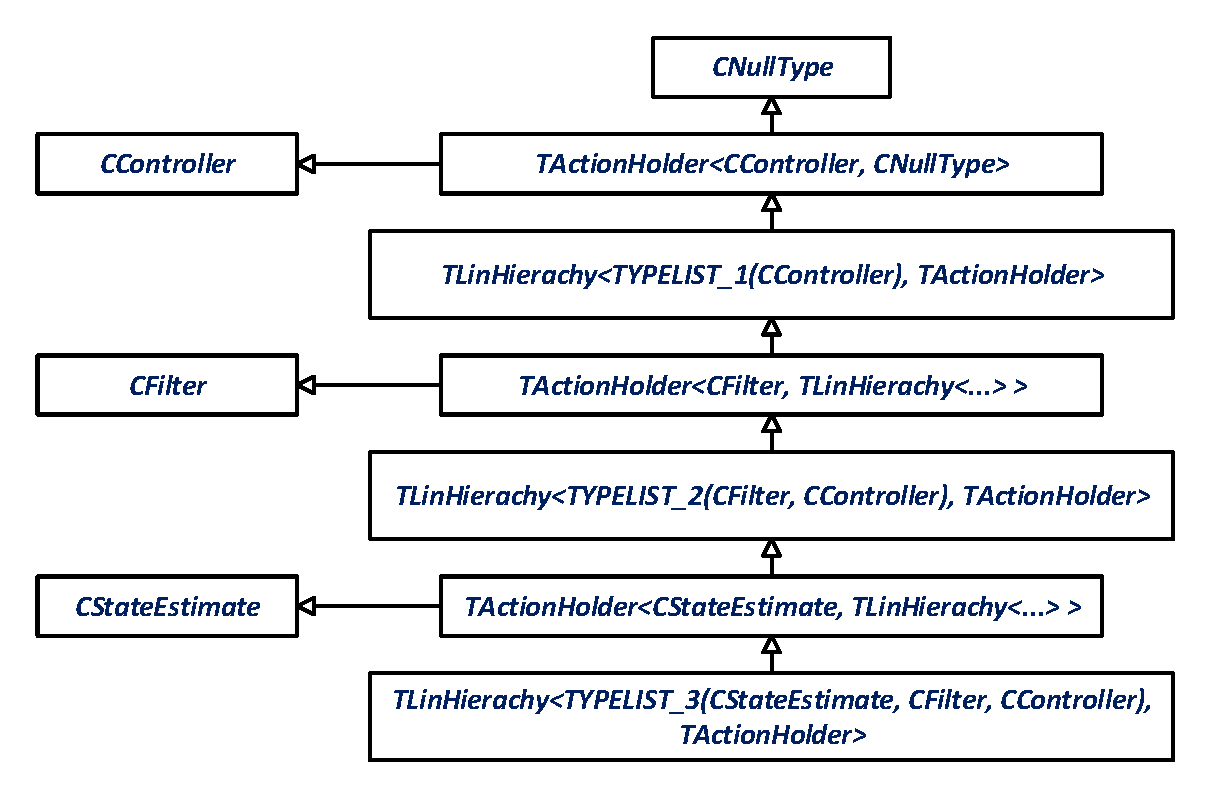
\includegraphics[width=0.7\linewidth]{img/SW_1_Signalfluss_KD.pdf}
\caption{Klassendiagramm der generierten Hierarchie}
\end{figure}
Der Vorteil dieses Konzepts, welches mit einem nicht zu vernachlässigenden Programmieraufwand verbunden ist, zeigt sich bei der letztendlichen Nutzung. Sind die Aktionsobjekte definiert, können sie in wenigen Zeilen zu dem Signalfluss zusammengesetzt werden.
\begin{lstlisting}[caption={Anwendungsbeispiel der linearen Hierarchie},captionpos=b]
using ActionList = TYPELIST_3(CStateEstimate, CFilter, CController);
using SignalFlow = TLinHierachy<ActionList, TActionHandler>;
SignalFlow mySF;
\end{lstlisting}
Sollen nun im Projektverlauf einzelne Elemente ausgetauscht oder erweitert werden, muss lediglich die Typendefinition von \textit{ActionList} geändert werden. Da die Hierarchie mittels Vererbung realisiert wird, können durch die Angabe des Namensraum die Methoden aller Elternklassen verwendet werden. Beispielsweise zeigt der folgende Ausschnitt die Abfrage aller berechneten Signale.
\begin{lstlisting}[caption={Beispiel für den Zugriff auf Aktionsobjekte in der Hierarchie},captionpos=b]
SStateVector x_estimate = mySF.CStateEstimate::getValue();
SStateVector x_filtered = mySF.CFilter::getValue();
UType        u          = mySF.CController::getValue();
\end{lstlisting}
Ebenso können zur Laufzeit konfigurierbare Elemente oder Verzweigungen implementiert werden. Angenommen zur Filterung sollen entweder ein Komplementär-Filter (\textit{CCompFilter}) oder ein Tiefpass erster Ordnung (\textit{CPT1}) genutzt werden, kann eine Klasse \textit{CFilterSystem} aus diesen beiden komponiert werden, die zusätzliche Methoden zur Filterauswahl bietet.
\begin{lstlisting}[caption={Beispiel für die komponierte Aktionsobjekte},captionpos=b]
class CFilterSystem
{
public:
	using InputType  = SStateVector;
	using OutputType = SStateVector;
public:
	const OutputType& calcOutput(const InputType& input)
	{
		mCompFilter.calcOutput(input);
		mPT1Filter.calcOutput(input);
		
		return this->getValue();
	}
	const OutputType& getValue()
	{
		switch(mActiveFilter)
		{
			case EFilter::CompFilter:
				return mCompFilter.getValue();
			case EFilter::PT1Filter:
				return mPT1Filter.getValue();
			default:
				return input;
		}
	}
	void setFilter(EFilter filter)
	{
		mActiveFilter = filter;
	}
private:
	CCompFilter mCompFilter;
	CPT1        mPT1Filter;
	EFilter     mActiveFilter;
};
\end{lstlisting}
Analog können auch komplexere Verzweigungen realisiert werden, wobei \textit{TLinHierachy} zur Generation von Teilzweigen des Blockschaltbildes verwendet werden kann.